\chapter{Implementácia}

\section{Vývoj s pomocou príkazového riadku}

Ruby on Rails má zabudovanú konzolovú aplikáciu, ktorá uľahčuje vývoj pomocou príkazov. Ak zadáme \emph{\$ rails help} tak dostaneme nasledovný výstup

\begin{minted}{bash}
$ rails help
Usage: rails COMMAND [ARGS]

The most common rails commands are:
 generate    Generate new code (short-cut alias: "g")
 console     Start the Rails console (short-cut alias: "c")
 server      Start the Rails server (short-cut alias: "s")
 test        Run tests (short-cut alias: "t")
 dbconsole   Start a console for the database specified in config/database.yml
             (short-cut alias: "db")
 new         Create a new Rails application. "rails new my_app" creates a
             new application called MyApp in "./my_app"

 ...
\end{minted}

\clearpage
Tieto príkazy dokážu urýchliť vývoj, keďže nemusíme konfigurovať štruktúru adresárov, sťahovať repozitáre Ruby on Rails a vytvárať súbory ručne alebo poskytuje iné nástroje.
Najdôležitejšie pri vývoji sú príkazy \emph{rails server}, \emph{rails console} a \emph{rails new}. 


\textbf{\emph{\$ rails server}} -- ako meno napovedá spustí server, ktorý je určený v súbore balíčkov -- \emph{Gemfile}, pričom môžeme flagmi špecifikovať na akom porte a adrese sa má aplikácia spustiť.

\textbf{\emph{\$ rails console}} -- spúšťa interaktívnu konzolu, kde vývojár môže otestovať správanie jednotlivých komponentov webovej apliácie, bez toho aby musel spúšťať server a testovať cez užívateľské rozhranie v prehliadači.

\textbf{\emph{\$ rails new my\_app}} -- sa nepoužíva príliš často, keďže tento príkaz vytvára novú aplikáciu aj s celou jej štruktúrou. Zároveň nastaví a stiahne všetky závislosti. Pri vytváraní sa môžu určité závislosti, ako použitá databáza alebo použitý JavaScript-ový framework pomocou flagov (napríklad \emph{-d=postgresql} ak chceme použiť pri všetkých štádiach vývoja databázu PostgreSQL.

Ďalšia časť príkazov sú generátory súborov ako bolo spomenuté v kapitole 2.2. Generátory vytvárajú iba kostru súboru spolu aj s názvom, kde potom vývojar môže dopísať svoj kód. Všetky typy generátorov súborov môžeme zobraziť pomocou príkazu \emph{\$ rails generate}.

Dôležité príkazy sú pre prácu s migráciami a teda databázou. Keď má vývojár migrácie napísané tak ich potrebuje aby sa podľa nich v databáze vytvorili tabuľky, stĺpce, indexy... Príkazov pre prácu s databázou je mnoho ale pri vývoji som používal najčastejšie nasledujúce:

\begin{minted}{bash}
$ rails db:[COMMAND]
$ rails db:create   # Vytvorí databázu
$ rails db:migrate  # Prevedie všetky migrácie z DSL do databázy
$ rails db:seed     # Vytvorí prichystané objekty do databázy
                    # zo súboru ./db/seeds.rb
$ rails db:rollback # Vráti všetky zmeny z predchádzajúcej migrácie
$ rails db:drop     # Odstráni databázy
\end{minted}

\section{Smerovanie}

Ruby on Rails využíva pri mapovaní URL adries router. Tieto mapovania môže vývojár ľubovoľne meniť a teda priradiť určitú cestu danému controller-u. Všetky tieto cesty sídlia v súbore \emph{./config/routes.rb}. Cesty môžeme priebežne sledovať aj pomocou príkazu \emph{\$ rails routes}. Tu je ukážka definovaných ciest z aplikácie pre podporu rozvrhov:

\begin{minted}{ruby}
Rails.application.routes.draw do
  root "pages#index"
  devise_for :users

  namespace :api do
    post "/teacher/group/course", to: "teacher_group_courses#create"
    delete "/teacher/group/course", to: "teacher_group_courses#destroy"
  end

  resources :courses
  resources :groups
  resources :teachers do
    resources :reports, controller: "teacher_reports" do
      get "/email", to: "teacher_reports#email"
      post "/email", to: "teacher_reports#email_send"
    end
  end
  ...
end
\end{minted}

Existuje niekoľko príkazov ktoré tieto cesty umožňujú vytvárať pomocou a sú nazvané podľa typu HTTP requestu (GET, POST). Keď sú cesty definované pomocou týchto funkcií majú tvar:

\begin{minted}{ruby}
get "/stranka", to: "controller#akcia"
\end{minted}

Kde hash \emph{to: STRING} mapuje cestu na špecifický controller a akciu v ňom. Sú však aj ďalšie špecifické prípady, napríklad domovská stránka aplikácie sa definuje pomocou funkcie \emph{\texttt{root "controller\#akcia"}}

Príkaz \emph{\texttt{resources :symbol}} je v skratkou pre vytváranie REST-ful ciest a cesty vygenerované týmto príkazom vyzerajú nasledujúco:

\begin{minted}{bash}
       NAZOV VERB   CESTA                 CONTROLLER#AKCIA
symbol_index GET    /symbol               symbol#index
             POST   /symbol               symbol#create
  new_symbol GET    /symbol/new           symbol#new
 edit_symbol GET    /symbol/:id/edit      symbol#edit
      symbol GET    /symbol/:id           symbol#show
             PATCH  /symbol/:id           symbol#update
             PUT    /symbol/:id           symbol#update
             DELETE /symbol/:id           symbol#destroy
\end{minted}

V príklade môžeme vidieť aj preddefinovaný príkaz \emph{devise\_for :users}, ktorý je súčasťou balíčka autentifikácie užívateľov nazvaného Devise a vytvára cesty potrebné pre fungovanie tohto balíčka.

Ďalej je použitá aj funkcia \emph{namespace :api ...}, ktorá dokáže zoskupovať podobné príkazy pod spoločnú url, v príklade je to api, čiže všetky cesty budú začínať \emph{\texttt{\/api/cesta}}.

\section{Modely}

Všetky modely aplikácie prebývajú v adresári \emph{./app/models}. Modely ako také vyzerajú jednoducho (príklad z aplikácie):

\begin{minted}{ruby}
class Teacher < ApplicationRecord
  has_many :teacher_courses
  has_many :courses, through: :teacher_courses

  has_many :teacher_group_courses
  has_many :groups, through: :teacher_group_courses

  has_many :documents

  validates :name, presence: true
  validates :email, presence: true

  def lecturer_ids
    ids = 
      self.teacher_courses
          .select{ |c| c.is_lecturer }
          .map{ |i| i.course_id}
  end
end
\end{minted}

Tento model predstavuje vyučujúceho v systéme. Vidíme, že model dedí väčšinu svojho správania z abstraktnej triedy \emph{ApplicationRecord}, ktorá dedí všetko správanie z \emph{ActiveRecord::Base}, preto nebotrebuje definovať skoro žiadne metódy a všetky atribúty tohto objektu sú definované v migrácii a nezavadzajú v súbore modelu. 

V príklade ako prvé môžeme vidieť definovanie vzťahov M:N a 1:N pomocou funkcíí \emph{has\_many} a \emph{has\_many} s hashom \emph{through: :symbol} kde sa definuje vzťah M:N a v ktorej tabuľke sa má vytvoriť prepojenie.

Ďalšie kľúčové funkcie v príklade sú \emph{\texttt{validates :attribute, \{opts\}}} ktoré vykonávajú validáciu atribútov (v príklade konkrétne, či sú prítomné) vždy pred uložením dát do databázy. Ak validácie zlyhajú tak dáta nie sú uložené.

Ako posledná je v príkladovom modeli definovaná pomocná funkcia na parsovanie id prednášajúcich jednotlivých predmetov. 

\section{Controllers}

Controllery sú najdôžežitejšia časť aplikácie, keďže načítajú dáta z databázy pomocou modelov, zavolajú view, ktorý dáta vykreslí a nakoniec sa vráti výsledok používateľovi. Prejdeme jednotlivé časti controller-a predmetov ktorý je súčasťou aplikácie. Nachádza sa v:

\begin{minted}{bash}
./app/controllers/courses_controller.rb
\end{minted}

Hneď po deklarácii triedy vidíme, že controller volá funkcie \emph{\texttt{before\_action}}, ktoré sa nazývajú filtre \citep{web:guides_filters}:

\begin{minted}{ruby}
before_action :find_course, only: [:show, :edit, :update, :destroy]
before_action :authenticate_user!
\end{minted}

Prvá funkcia, volá privátnu funkciu \emph{\texttt{find\_course}}, ktorá načíta do premennej inštancie predmet pomocou modelu a parametru id z tela HTTP požiadavky. Navyše, tento filter je obmedzený hashom \emph{only: [:show...]}, čo obmedzí pred ktorými akciami sa filter vyvolá. To nám zabezpečí, aby sme sa neopakovali pri jednotlivých akciách načítaním predmetu:

\begin{minted}{ruby}
private
def find_course
  @course = Course.find(params[:id])
end
\end{minted}

Ako môžeme vidieť aj v ostatné akcie využívajú objekt \emph{params}. V tomto objekte je uložené parsované telo HTTP požiadavky či už ide o GET alebo POST požiadavku a môžeme k jednotlivým položkám pristupovať pomocou symbolov.

Druhý filter volá funkciu \emph{\texttt{authenticate\_user!}}, ktorá je súčasťou balíčka \emph{Devise}, ktorý je použitý na autentifikáciu a tento filter zabezpečí, aby všetky akcie mohol využívať iba prihlásený užívateľ.

Ďalej v controller-i nasledujú jednotlivé akcie, ktoré sú namapované na URL adresy pomocou smerovača. Ako príklad zoberiem akciu \emph{create}:

\begin{minted}{ruby}
def create
  @course = Course.new(course_params)

  if @course.save
    flash[:notice] = "Predmet #{@course.name} bol úspešne vytvorený"
    redirect_to courses_path
  else
    render 'new'
  end
end
\end{minted}

Akcia začína tým, že sa vytvorí nový objekt s pomocou funkcie \emph{\texttt{course\_params}}. Táto funkcia je definovaná na konci súboru controller-a ako privátna metóda:

\begin{minted}{ruby}
def course_params
  params.require(:course)
        .permit(:code, :name, :lectures_weekly, 
                :classes_weekly, :lab_classes_weekly)
end
\end{minted}

Funkcia zaručí, že vráti z objektu \emph{params} iba tie parametre, ktoré povolíme a zadáme do funkcie \emph{.permit(...)}, čím obráni aplikáciu pred nechcenými vstupmi od koncového užívateľa.

Ďalej v tele akcie nasleduje kontrola stavu uloženia. Ak je v modeli všetko v poriadku, validácie prebehnú správne a nevyskytne sa žiadna chyba funkcia nastaví do session jednorázový odkaz, že predmet bol úspešne vytvorený a presmeruje užívateľa na zoznam všetkých predmetov. Ak pri uložení niečo zlyhalo tak sa iba zobrazí formulár ako pri vytváraní predmetu avšak už s vyplnenými hodnotami z predchádzajúceho pokusu (ak nie je definované, že atribút sa nemá zapamätať, ako napríklad heslo).

Na tomto princípe fungujú a majú podobnú štruktúru všetky controller-y a pri vývoji aplikácie som sa vo všetkých controller-och snažil dodržiavať vzor nazvaný REST (Representational state transfer). Ktorý pomáha vytvárať jednotné rozhrania pre webové aplikácie.

\section{Views}

Všetky viewy v Ruby on Rails aplikáciach sú uložené v adresári \emph{\texttt{.\/app\/views}} kde sú potom zaradené do respektívnych pod-adresárov podľa akcie v ktorej budú zobrazené. Každý view začína spoločnou šablónou (layout), ktorá je definovaná (pokiaľ nie je bližšie špecifikované) v súbore:

\begin{minted}{bash}
./app/views/layouts/application.html.erb
\end{minted}

View-y v Ruby on Rails využívajú pri šablónach formát ktorý sa volá Embedded RuBy -- a teda končí koncovkou ERB. Tento formát nám poskytuje funkcionalitu, kde môžeme vkladať kúsky kódu Ruby do obyčajného HTML dokumentu.

Ďalšia dôležitá funkcionalita je, že všetky premenné inštancie (@var) controller-a sú automaticky prítomné aj v rendrovanom view-e.

Potom ako sa view v Ruby on Rails vykreslí je vložený do hlavnej šablóny. Môžeme view-y ďalej rozširovať aj pomocou funkcie \emph{render}, ktorá môže rendrovať čiastočné view-y ako napríklad formuláre. V aplikácii máme príklad, render formuláru predmetu:

\begin{minted}{erb}
<h1>Upraviť predmet <%= @course.name %></h1>
<%= render 'form', course: @course %>
<%= link_to "Späť", courses_path %>⏎
\end{minted}

V prvom riadku príkladu je samozrejme vypísanie nadpisu úrovne H1 kde je zároveň uvedené aj meno predmetu. Ďalší riadok používa metódu render, ktorá vykreslí čiastočný view s menom \emph{\_form} (všetky čiastočné view-y musia začínať s podtržníkom) pričom mu predáva premennú predmetu. V tretiom riadku vidíme pomocnú funkciu na generovanie linku, kde sa použije meno cesty.

\clearpage
\begin{minted}{erb}
<%= form_for course do |f| %>
    <%= render 'layouts/errors', model: course %>

    <div class="form-group">
        <%= f.label "Kód predmetu" %>
        <%= f.text_field :code, class: "form-control" %>
    </div>

    <div class="form-group">
        <%= f.label "Meno predmetu" %>
        <%= f.text_field :name, class: "form-control" %>
    </div>
    ...
\end{minted}

Toto je úryvok z obsahu súboru \emph{\texttt{courses/\_form.html.erb}}. Prvá vec ktorú si všimneme je že predmet (\emph{course}) už nie je premennou inštancie ale iba lokálnou premennou, ktorá je použitá vo helper funkcii \emph{\texttt{form\_for}}, ktorá uľahčuje tvorbu formulárov.

\begin{minted}{erb}
<tbody>
    <% @courses.each do |course| %>
      <tr>
        <td><%= course.code %></td>
        <td><%= course.name %></td>
    ...
\end{minted}

Veľmi dôležitou funkciou je aj prechádzanie cez kolekciu objektov. To docielime jednoducho použitím funkcie \emph{.each} priamo na kolekciu objektov kde môžeme potom k jednotlivým elementom pristupovať v príslušnom bloku.

\section{Generovanie PDF prehľadov}

Generovanie PDF dokumentov zabezpečuje balíček \emph{\texttt{wicked\_pdf}}, ktorý je wrapper pre aplikáciu v príkazovom riadku \emph{\texttt{wkhtmltopdf}}. Dokáže prekonvertovať HTML dokument do PDF dokumentu, pričom sa dá naštýlovať dokument naštýlovať pomocou CSS a dokonca aj JavaScriptom. 

V prvej verzii implementácie sa PDF prehľady generovali priamo v okne užívateľa, ale keďže generovanie PDF dokumentov je časovo náročnejšie, užívateľ bol nútený čakať kým sa dokument zobrazí/stiahne. Nakoniec som tento problém vyriešil použitím balíčka \emph{\texttt{delayed\_job}}. Viac o tom to riešení píšem v sekcií \ref{sec:request_time}

\section{Odosielanie e-mailov}

Ruby on Rails obsahuje v základe zabudovanú funkcionalitu na odosielanie a prijímanie emailov nazvanú \emph{Action Mailer}. Ten poskytuje generátor súborov a teda jednoduchý základ pre vývojára. Všetky súbory na prácu s emailami sú uložené v adresári \emph{\texttt{./app/mailers}} a šablóny emailov sú umiestnené v \emph{\texttt{./app/views}}. Tu je príklad ako sa odosielajú e-maily spolu aj s prehľadom vyučujúceho v prílohe vo formáte pdf:

\begin{minted}{ruby}
def mail_teacher_report(teacher, document, subject, body)
  @teacher = teacher
  @body = body
  
  attachments[document.filename] = File.read(
    Rails.root.join("pdfs", document.filename)
  )

  mail(to: @teacher.email, subject: subject)
end
\end{minted}

Premenné, ktoré sa pošlú do funkcie mailera \emph{\texttt{mail\_teacher\_report}} sprístupníme šablóne e-mailu tým, že ich priradíme do premenných inštancie. Ďalej do poľa \emph{attachments} načítame súbor priamo z adresára, kde sú súbory pdf uložené. Nakoniec odošleme e-mail pomocou funkcie mail, kde nastavíme hash pre koho je e-mail určený a predmet e-mailu.

Potrebujeme ale definovať, kedy sa má tento e-mail odoslať a to môžeme spraviť priamo v controller-i. Keď užívateľ vyžiada aby bol email odoslaný tak v akcií controllera zavoláme daný mailer a funkciu, ktorá je na to určená:

\begin{minted}{ruby}
ReportMailer.mail_teacher_report(@teacher, @document, @subject, @body)
            .deliver_later
\end{minted}

V príklade je uvdená funkcia \emph{\texttt{deliver\_later}} ktorá odošle e-mail na pozadí bez toho aby zdržovala priebeh spracovania požiadavku. Môžeme však aj definovať funkciu \emph{\texttt{deliver\_now}}, ktorá bude čakať na odoslanie e-mailu a teda blokovať spracovanie požiadavky.

\clearpage
\section{Užívateľské rozhranie}

\subsection{Prihlásenie a registrácia}

Pred začatím používania aplikácie sa musí užívateľ najprv prihlásiť alebo registrovať. Všetky podstránky aplikácie sú zabezpečené a užívateľ je presmerovaný pokiaľ nie je prihlásený.

\begin{figure}[!htb]
  \centering
  %\hspace*{-1cm}
  %\includegraphics[width=1.1\textwidth]{content/images/login}
  \includegraphics[width=1\textwidth]{content/images/ui/login}
  \caption{Rozhranie pre prihlásenie do aplikácie.}
\end{figure}

Užívatelia si taktiež môžu prenastaviť heslo pomocou emailu ak ho náhodou zabudli. Na zadaný email sa zašle link na stránku, kde užívateľ môže heslo zmeniť. Registrácia sa navyše dá kedykoľvek vypnúť administrátorom použitím premennej prostredia.

\clearpage
\subsection{Predmety a skupiny}

\begin{figure}[!htb]
  \centering
  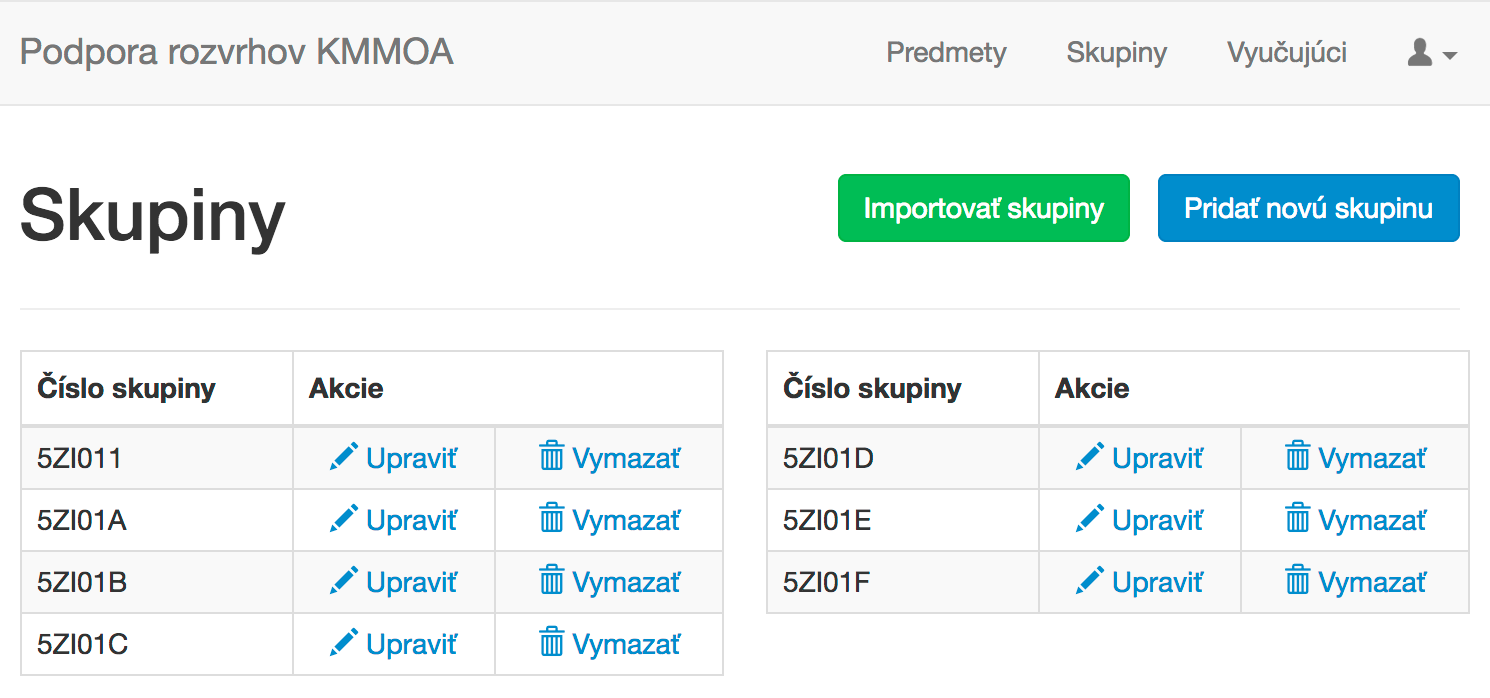
\includegraphics[width=1\textwidth]{content/images/ui/groups}
  \caption{Prehľad skupín.}
  \label{fig:groups}
\end{figure}

\begin{figure}[!htb]
  \centering
  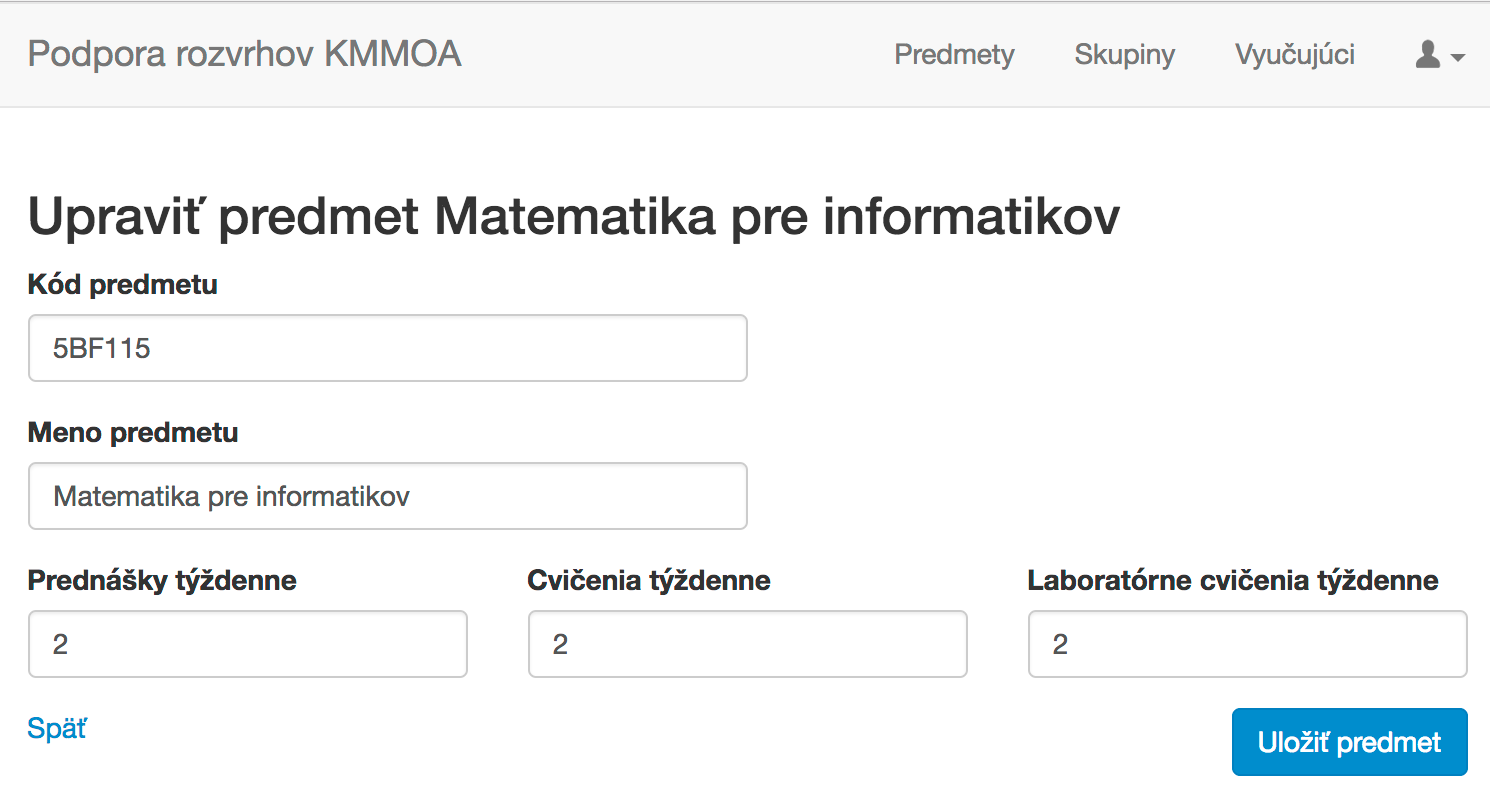
\includegraphics[width=1\textwidth]{content/images/ui/course_edit}
  \caption{Formulár predmetu (úprava).}
  \label{fig:courses}
\end{figure}

\clearpage
Prehľad predmetov vyzerá podobne ako na obrázku (obr. \ref{fig:groups}). Prehľady sú zobrazené buď v jednej alebo dvoch tabuľkách vedľa seba podľa počtu údajov v aplikácii, pričom pri každom zázname je možnosť ho upraviť alebo zmazať a nad tabuľkou je tlačidlo, ktoré umožňuje pridať nové záznamy a pri skupinách je možnosť ich importovať z CSV súboru. 

Formuláre skupín a predmetov sú podobné, pričom formulár skupín obsahuje aj \emph{Select box} kde užívateľ môže danej skupine priradiť predmety.

\subsection{Vyučujúci}

\begin{figure}[!htb]
  \centering
  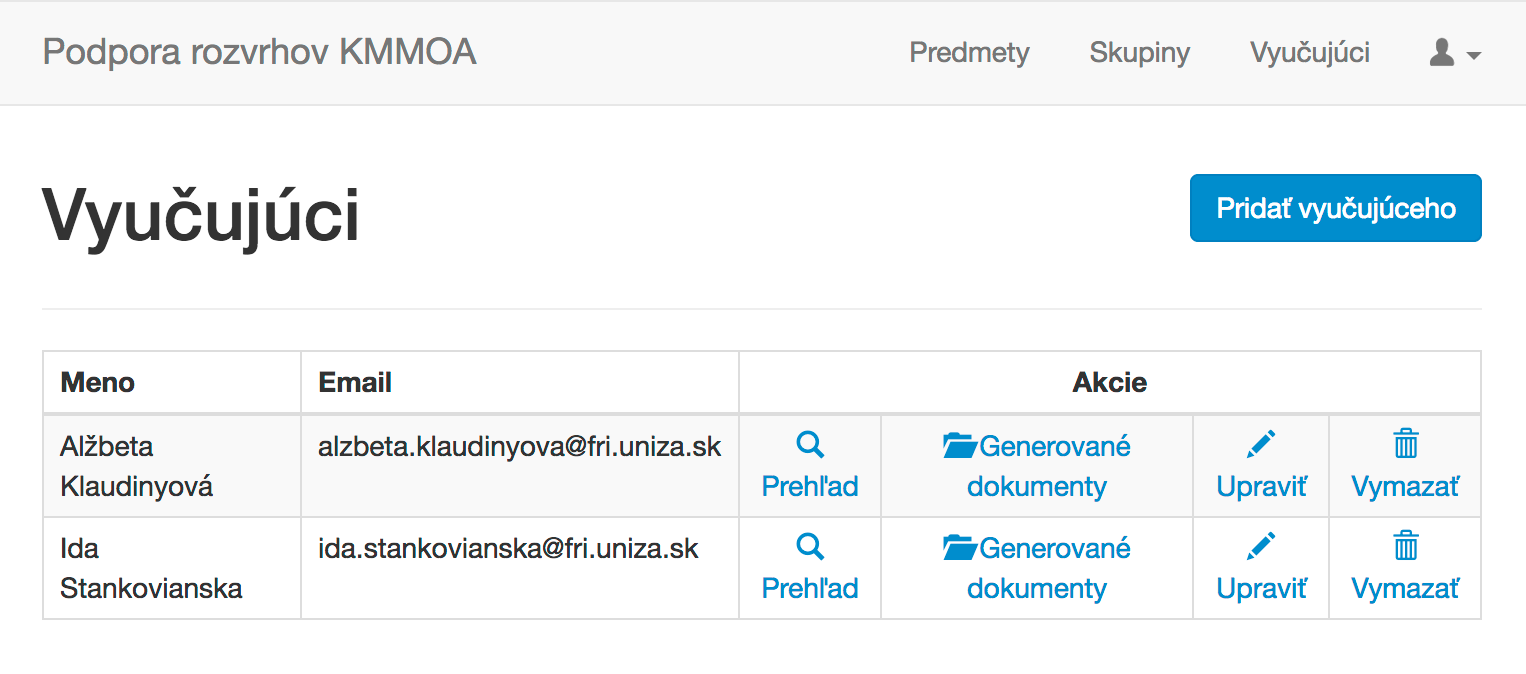
\includegraphics[width=1\textwidth]{content/images/ui/teachers}
  \caption{Prehľad vyučujúcich.}
  \label{fig:courses}
\end{figure}

Prehľad vyučujúcich obsahuje okrem pridania, úpravy a vymazania taktiež prehľad, kde užívateľ môže prezrieť aktuálny prehľad bez toho aby sa musel generovať PDF dokument a v generovaných dokumentoch je celá história vygenerovaných dokumentov. V prehľade dokumentov (obr. \ref{fig:reports}) môže užívateľ vidieť stav generovania a počet odoslaní emailov (ak bol dokument odoslaný), prípadne si môže dokumenty zobraziť a aj ich odoslať, kde len vyplní predmet, telo e-mailu a dokument bude automaticky priložený ako príloha.

\clearpage
\begin{figure}[!htb]
  \centering
  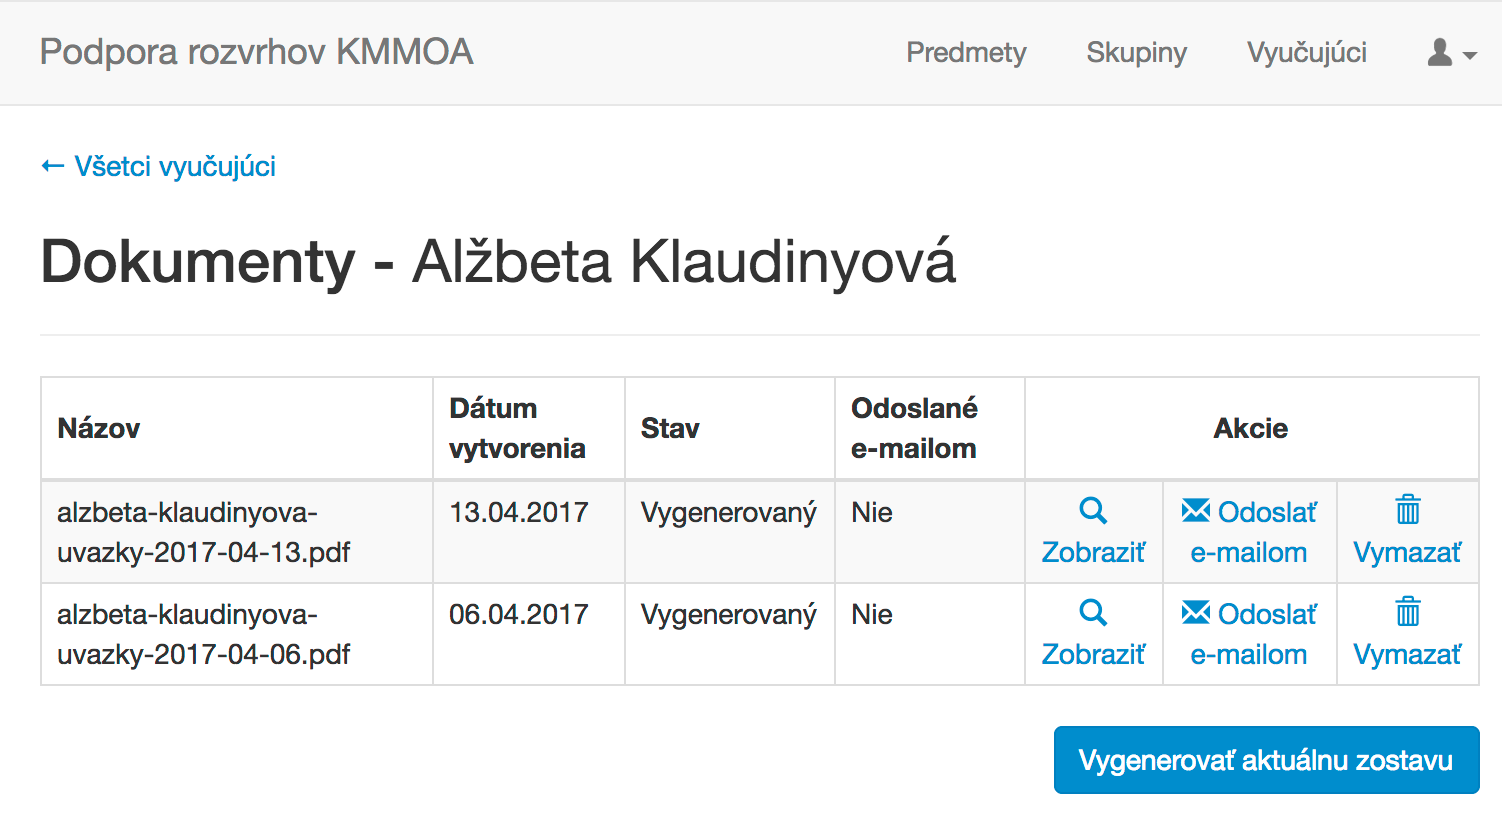
\includegraphics[width=1\textwidth]{content/images/ui/reports}
  \caption{Prehľad dokumentov.}
  \label{fig:reports}
\end{figure}

Úprava vyučujúceho vyzerá zložitejšie oproti predchádzajúcim formulárom, ale obsahuje iba zopár polí. Užívateľ musí zvoliť, ktoré predmety daný vyučujúci vyučuje, po čom sa následne zobrazia skupiny, ktoré majú priradené tieto predmety a môže následne priradiť ktoré skupiny predmetu vyučujúci vyučuje. Zároveň môže užívateľ označiť pole Select box ``Je prednášajúci'', čo sa odzrkadlí na prehľade úväzkov vyučujúceho (obr. \ref{fig:teacher_show}).

Prehľad úväzkov vyučujúceho navyše využíva čiastočný view, ktorý je použitý aj pri vykreslení a konverzii prehľadu do PDF súboru.

\begin{figure}[!htb]
  \centering
  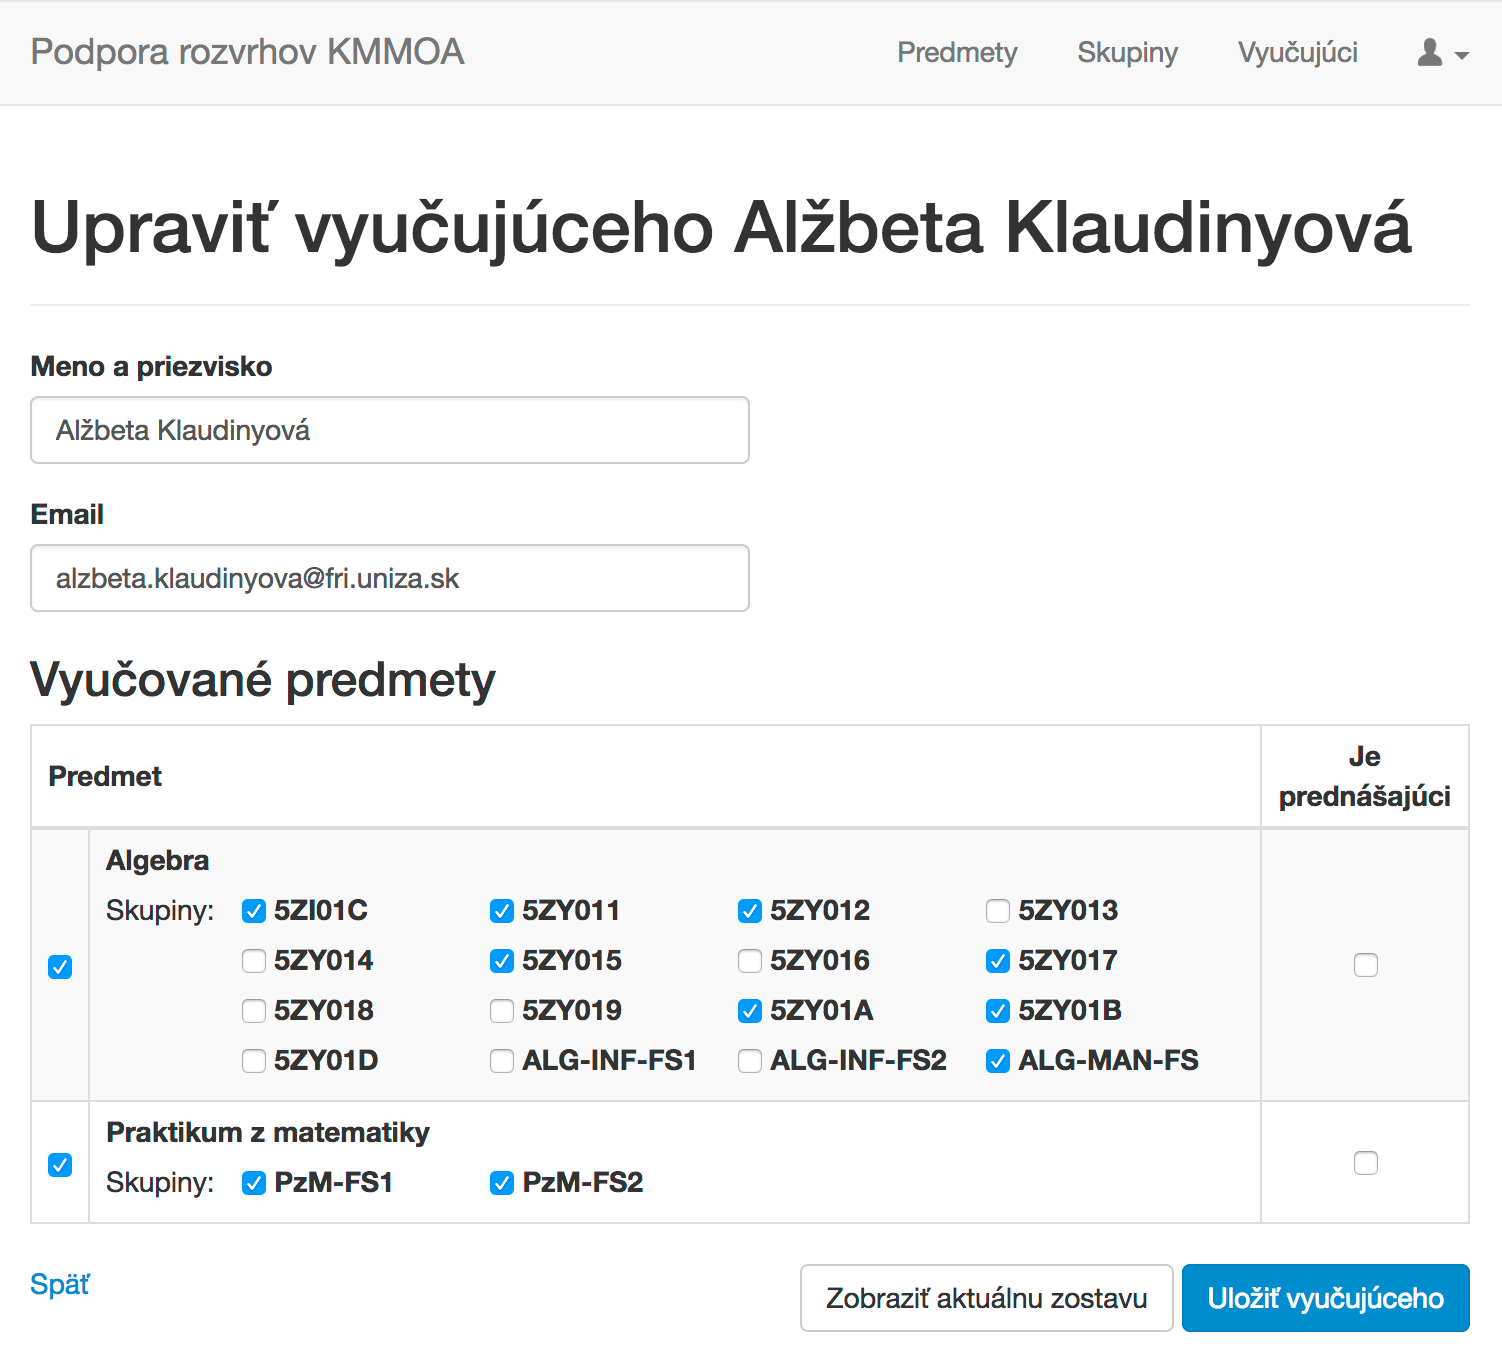
\includegraphics[width=1\textwidth]{content/images/ui/teacher_edit}
  \caption{Úprava vyučujúceho.}
  \label{fig:teacher_edit}
\end{figure}

\begin{figure}[!htb]
  \centering
  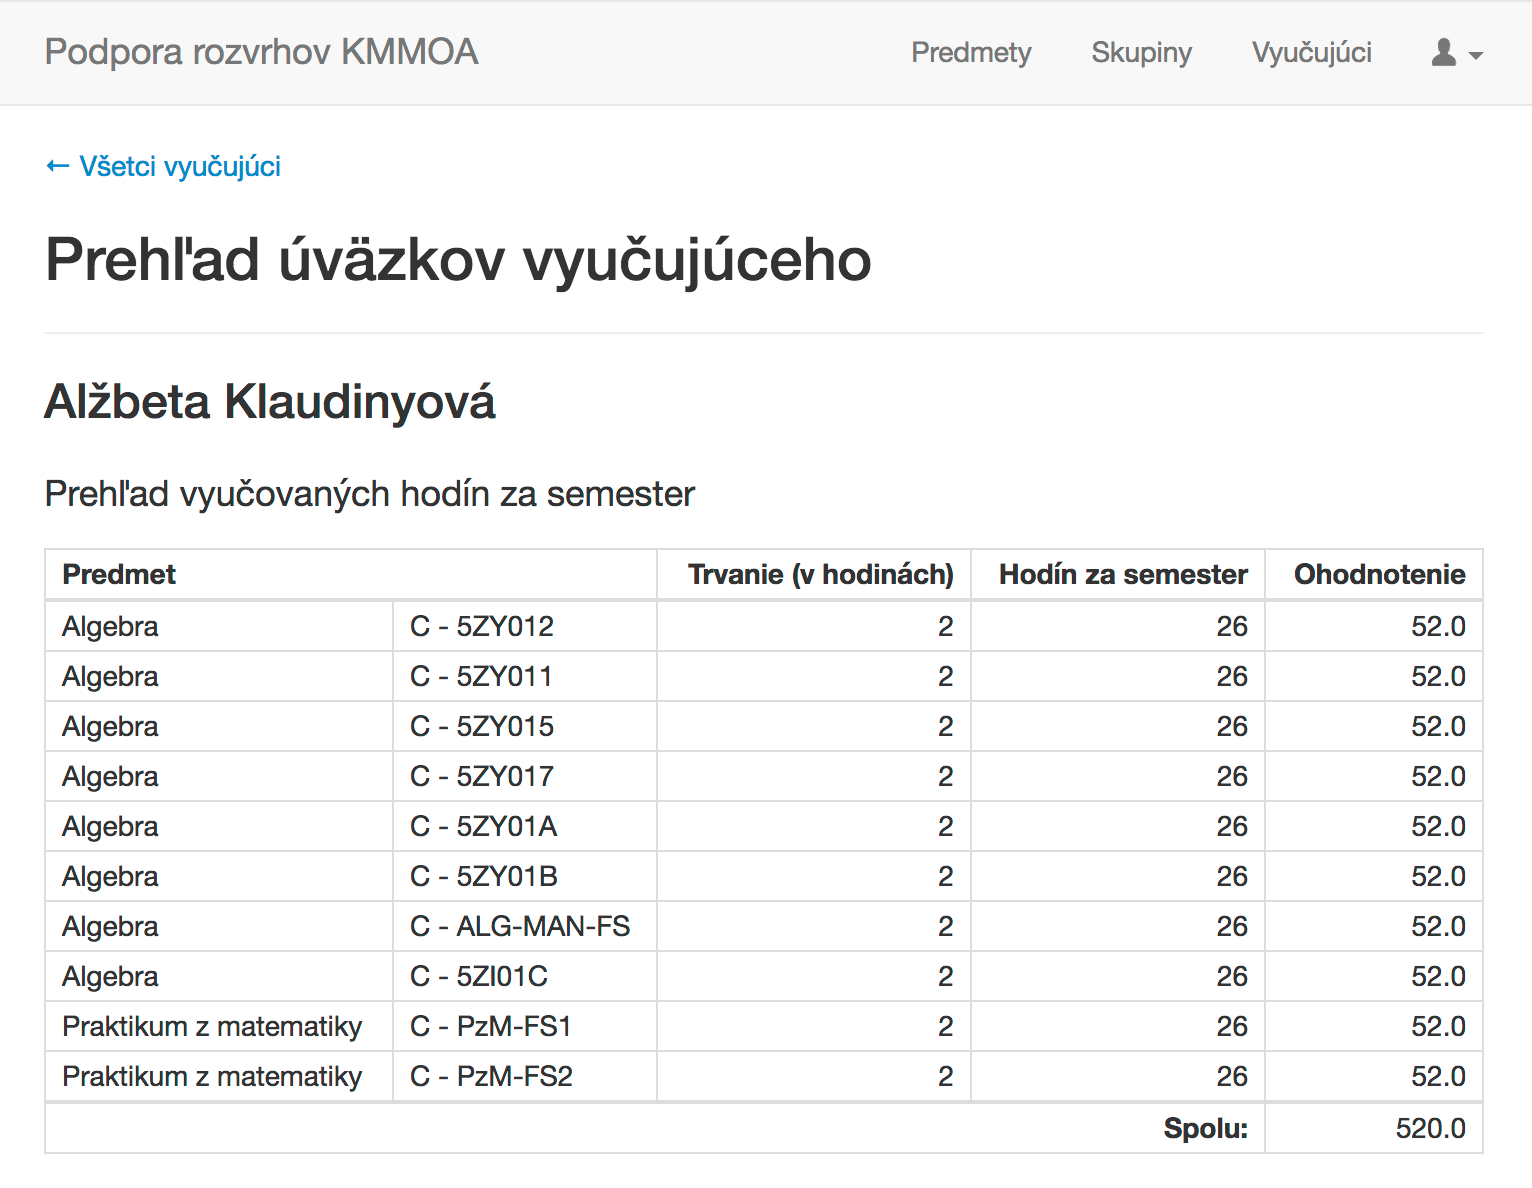
\includegraphics[width=1\textwidth]{content/images/ui/teacher_show}
  \caption{Prehľad úväzkov vyučujúceho.}
  \label{fig:teacher_show}
\end{figure}


\clearpage
\section{Turbolinks}

Turbolinks je JavaScript knižnica, ktorá robí navigáciu po webovej stránke rýchlejšou. Poskytuje rýchlostné benefity single-page aplikácie, bez pridanej komplexnosti iných JavaScript frameworkov. Vykreslenie celej HTML stránky môže bez obáv prebiehať na strane servera. Keď chce užívateľ prejisť na inú stránku pomocou kliknutia na link Turbolinks pomocou AJAX-u vyzdvihne danú stránku a vymení obsah tagu \emph{<body>} a zlúči obsah v tagoch \emph{<head>}, to všetko bez potreby znovu načítať celú stránku. \citep{web:turbolinks}

\section{Problémy pri implementácii a ich riešenie}
\subsection{N+1 queries}

Pri načítaní niektorých prehľadov, ako napríklad prehľad vyučujúcich sa začali v logoch servera objavovať dlhé zoznamy SQL dotazov. Ako prvé som si všimol, že je to spôsobené iteráciou cez vzťahy kolekcie modelov. Ako napríklad:

\begin{minted}{ruby}
@techers = Teacher.all()

@teachers.courses.each do |course|
  puts course.title
end
\end{minted}

To spôsobí, že pre každý model vo vzťahu je načítaný samostatným SQL selectom, čo ale nechceme, pretože to spôsobuje nadmerné zaťaženie databázy. Po zamyslení nad týmto problémom je jasné, že musíme načítať modely aj všetky ich vzťahy cez ktoré chceme iterovať naraz s použitím JOIN-u.
Našťastie ale vývojári ActiveRecord-u na toto správanie mysleli a nezabudli ho implementovať. Riešenie je veľmi jednoduché:

\begin{minted}{ruby}
@techers = Teacher.includes(:courses).all()

@teachers.courses.each do |course|
  puts course.title
end
\end{minted}

Pri načítaní modelov použijeme funkciu \emph{includes()} do ktorej môžeme napísať symboly, ktoré reprezentujú jednotlivé vzťahy. Po skontrolovaní logov teraz vidíme, že pri načítaní náhľadu sa teraz spustí iba 1 SQL query.

\subsection{Dlhé časy požiadaviek}
\label{sec:request_time}

Toto správanie je spôsobené tým, že funkcia v controlleri trvá dlhšie ako je obvyklé a tým zdržiava navrátatenie odpovede užívateľovi.
Problém sa vyskytol najmä pri odosielaní e-mailov a generovaní PDF prehľadov. Ide o jednoduchý problém, ktorý sa dá vyriešiť niekoľkými spôsobmi. 

V aplikácii je tento problém vyriešený použitím balíčka (\emph{\texttt{gem 'delayed\_job'}}), ktorý vykonáva dlho-trvajúce funkcie na pozadí. Balíček má v databáze svoju tabuľku, do ktorej ukladá všetky funkcie, ktoré má vykonať. 

Avšak, tento balíček sa musí spustiť externe cez príkazový riadok, preto je múdre pridať aj balíček (\emph{\texttt{gem 'daemons'}}) aby sme mohli tento proces daemonizovať. Spustíme ho zo zložky aplikácie príkazom:

\begin{minted}{bash}
$ bin/delayed_job start
\end{minted}

Neskôr treba na produkčnom serveri tento skript nalinkovať aby sa automaticky spúšťal pri štarte/reštarte servera.